\documentclass[aspectratio=169, 11pt]{beamer}

% --- USER-REQUESTED THEME ---
\usetheme{Goettingen}
\usecolortheme{default}
\setbeamertemplate{navigation symbols}{} % Hides the navigation symbols

% --- PDFLATEX COMPATIBLE PREAMBLE ---
\usepackage[utf8]{inputenc}
\usepackage[T1]{fontenc}
\usepackage[english]{babel}

% Math and symbols packages
\usepackage{amsmath,amsfonts}
\usepackage{amssymb}
\usepackage{graphicx}
\usepackage{booktabs}
\usepackage{braket}
\usepackage{physics} 
\usepackage{wasysym} 
\usepackage{array}  
\usepackage{tikz}
\usetikzlibrary{shapes, arrows, positioning, calc, decorations.pathreplacing}
% TikZ Style Definitions
\tikzset{
    block/.style = {rectangle, draw, fill=blue!20, text width=5em, text centered, rounded corners, minimum height=4em},
    wideblock/.style = {rectangle, draw, fill=blue!20, text width=8em, text centered, rounded corners, minimum height=3em},
    line/.style = {draw, -latex', thick},
    cloud/.style = {draw, ellipse, fill=red!20, node distance=3cm, minimum height=2em, align=center},
    decision/.style = {diamond, draw, fill=green!20, text width=4.5em, text badly centered, node distance=3cm, inner sep=0pt}
}

% --- ADD PAGE NUMBERS ---
\setbeamertemplate{footline}
{
  \leavevmode%
  \hbox{%
    \begin{beamercolorbox}[wd=\paperwidth,ht=2.25ex,dp=1ex,right]{page number}%
      \usebeamerfont{page number}\insertframenumber{} / \inserttotalframenumber\hspace*{3ex}
    \end{beamercolorbox}%
  }%
  \vskip1pt%
}

% Metadata
\title[Predictive Algorithms for Quantum Materials]{Predictive Algorithms for Simulating Quantum Materials}
\subtitle{Tensor-D$\Gamma$A and Neural Nevanlinna}
\author[Chenan Wei]{Chenan Wei}
\date{Feb 4, 2026}

% Precise wording configurations
\setbeamertemplate{navigation symbols}{}
\setbeamertemplate{itemize items}[square]

\begin{document}

% Title Slide
\begin{frame}
    \titlepage
\end{frame}

% Outline
\begin{frame}{Outline}
    \tableofcontents
\end{frame}

% ==========================================
% NEW SECTION: Project Overview
% ==========================================
\section{Project Overview}

\begin{frame}{1.1 Motivation and Objectives}
    \textbf{The Goal:}
    To combine innovations in \textbf{tensor techniques} with \textbf{machine learning} to overcome the scaling limits of current \textit{ab initio} methods for correlated materials.
    
    \textbf{The Testbed: Strontium Ruthenate ($Sr_2RuO_4$)}
    \begin{itemize}
        \item A prototypical double bottleneck: High computational cost + experimental ambiguity.
        \item \textbf{Scientific Objective:} Definitively resolve the triplet vs singlet pairing mechanism debate.
        \item \textbf{Challenge:} Requires capturing non-local spin fluctuations in a 3-orbital system.
    \end{itemize}
\end{frame}

\begin{frame}{1.2 The Two Barriers}
    Currently, two specific barriers prevent predictive simulation of multi-orbital systems:
    
    \begin{columns}
        \column{0.48\textwidth}
        \begin{alertblock}{1. The Memory Barrier}
            \textbf{Context:} Diagrammatic extensions to DMFT (D$\Gamma$A) are needed for non-local fluctuations.
            \par
            \textbf{Problem:} The two-particle vertex $\Gamma^{\alpha\beta\gamma\delta}$ scales as $N_{orb}^4$. For $N_{orb} \ge 3$, this is too large for memory.
        \end{alertblock}
        
        \column{0.48\textwidth}
        \begin{alertblock}{2. The Noise Barrier}
            \textbf{Context:} Comparison with experiment requires Analytic Continuation.
            \par
            \textbf{Problem:} QMC noise is highly correlated. Standard optimization (MaxEnt/Nevanlinna) is brittle and over-smooths spectral features.
        \end{alertblock}
    \end{columns}
\end{frame}

\begin{frame}{1.3 Proposed Pipeline}
    \centering
    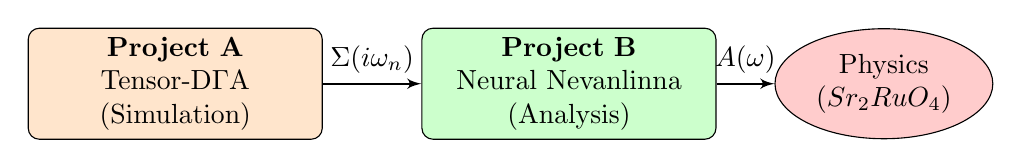
\begin{tikzpicture}[node distance=3cm, auto]
        \node [block, fill=orange!20, text width=3.5cm] (projA) {\textbf{Project A} \\ Tensor-D$\Gamma$A \\ (Simulation)};
        \node [block, right of=projA, node distance=5cm, fill=green!20, text width=3.5cm] (projB) {\textbf{Project B} \\ Neural Nevanlinna \\ (Analysis)};
        \node [cloud, right of=projB, node distance=4cm] (phys) {Physics \\ ($Sr_2RuO_4$)};
        
        \path [line] (projA) -- node[above] {$\Sigma(i\omega_n)$} (projB);
        \path [line] (projB) -- node[above] {$A(\omega)$} (phys);
    \end{tikzpicture}
    
    \vspace{1cm}
    \begin{itemize}
        \item \textbf{Project A:} Overcomes the memory barrier using Tensor Decompositions.
        \item \textbf{Project B:} Overcomes the noise barrier using Physics-Informed Neural Networks.
    \end{itemize}
\end{frame}

% ==========================================
% NEW SECTION: Project A
% ==========================================
\section{Project A: The Simulation Engine (Tensor-D$\Gamma$A)}

% --- NEW SLIDE: The Full Workflow ---
\begin{frame}{2.1 The Computational Pipeline: DMFT + D$\Gamma$A}
    \textbf{Concept:} We upgrade the local DMFT solution by adding non-local fluctuations in a post-processing step.
    
    \vspace{0.5cm}
    \centering
    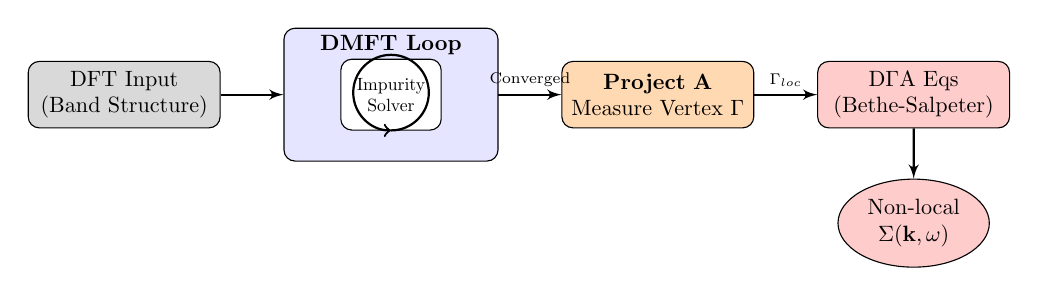
\begin{tikzpicture}[node distance=1.5cm, auto, scale=0.8, transform shape]
        % Nodes
        \node [wideblock, fill=gray!30] (dft) {DFT Input \\ (Band Structure)};
        
        % DMFT Loop container
        \node [wideblock, right=1cm of dft, fill=blue!10, minimum height=6em, text width=9em] (dmft) {};
        \node [anchor=north] at (dmft.north) {\textbf{DMFT Loop}};
        \node [block, fill=white, scale=0.8] at (dmft.center) (imp) {Impurity Solver};
        
        % Project A Node
        \node [wideblock, right=1cm of dmft, fill=orange!30, text width=8em] (measure) {\textbf{Project A} \\ Measure Vertex $\Gamma$};
        
        % DGammaA Node
        \node [wideblock, right=1cm of measure, fill=red!20] (dga) {D$\Gamma$A Eqs \\ (Bethe-Salpeter)};
        
        % Output
        \node [cloud, below=0.8cm of dga] (result) {Non-local \\ $\Sigma(\mathbf{k}, \omega)$};
        
        % Arrows
        \path [line] (dft) -- (dmft);
        \draw [line] (dmft.east) -- node[above, font=\scriptsize] {Converged} (measure.west);
        \path [line] (measure) -- node[above, font=\scriptsize] {$\Gamma_{loc}$} (dga);
        \path [line] (dga) -- (result);
        
        % Feedback loop drawing
        \draw [->, thick] (imp.south) arc[start angle=-90, end angle=270, radius=0.6cm];
    \end{tikzpicture}
    
    \vspace{0.5cm}
    \begin{itemize}
        \item \textbf{DMFT Step:} Converge the local self-energy $\Sigma_{loc}$ (Mott physics).
        \item \textbf{Project A:} Measure the massive 2-particle vertex on the \textit{frozen} impurity.
        \item \textbf{D$\Gamma$A Step:} Use $\Gamma$ to compute $\mathbf{k}$-dependent correlations (Spin fluctuations).
    \end{itemize}
\end{frame}

\subsection{Bottleneck}
\begin{frame}{2.1 The Vertex Bottleneck}
    To go beyond DMFT, we calculate the non-local susceptibility $\chi(\mathbf{q}, \omega)$ using the Bethe-Salpeter equation.
    
    $$ \chi(\mathbf{q}) = \left[ (\chi_0^{\mathbf{q}})^{-1} - \Gamma_{loc} \right]^{-1} $$
    
    \textbf{The Critical Obstacle:}
    \begin{itemize}
        \item The input is the local two-particle vertex $\Gamma_{loc}(\nu, \nu', \omega)$.
        \item Size $\propto N_{orb}^4 \times N_{freq}^3$.
        \item For a 3-orbital model ($Sr_2RuO_4$): This tensor is memory-prohibitive.
    \end{itemize}
\end{frame}

\subsection{Solution}
\begin{frame}{2.2 Solution: Tensor Train Decomposition}
    We exploit the low-rank structure of the vertex using Tensor Train (TT) decompositions (Matrix Product Operators).
    
    \textbf{Implementation Strategy:}
    \begin{enumerate}
        \item \textbf{On-the-fly Compression:} 
        Do not measure the dense tensor. Instead, implement a custom estimator in CT-QMC.
        \item \textbf{Direct Projection:}
        Project sampled configuration weights directly onto a compressed MPO manifold.
        \item \textbf{Result:}
        Bypass storage of the dense tensor entirely. Polynomial scaling vs Quartic scaling.
    \end{enumerate}
\end{frame}

\begin{frame}{2.3 Workflow: From QMC to Self-Energy}
    \centering
    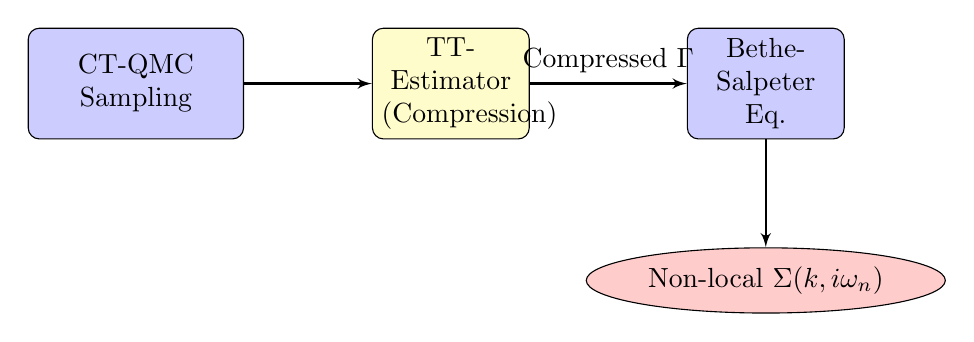
\begin{tikzpicture}[node distance=2.5cm, auto]
        % Nodes
        \node [block, text width=2.5cm] (qmc) {CT-QMC Sampling};
        \node [block, right of=qmc, node distance=4cm, fill=yellow!20] (tt) {TT-Estimator \\ (Compression)};
        \node [block, right of=tt, node distance=4cm] (bse) {Bethe-Salpeter Eq.};
        \node [cloud, below of=bse, node distance=2.5cm] (sigma) {Non-local $\Sigma(k, i\omega_n)$};

        % Edges
        \path [line] (qmc) -- (tt);
        \path [line] (tt) -- node[above] {Compressed $\Gamma$} (bse);
        \path [line] (bse) -- (sigma);
    \end{tikzpicture}
    
    \vspace{0.5cm}
    This output $\Sigma(k, i\omega_n)$ is the input for the analytic continuation framework (Project B).
\end{frame}

% ==========================================
% ORIGINAL CONTENT (Project B context)
% ==========================================
\section{Project B: Analysis Framework (Nevanlinna Theory)}

\begin{frame}{3.1 The Context: Analytic Continuation}
    \textbf{The Connection:}
    Project A yields the Green's function $G(i\omega_n)$ or Self-energy $\Sigma(i\omega_n)$ on the imaginary axis. To compare with experiments, we must map this to the real axis.

    \textbf{The Fundamental Relation:}
    \begin{equation}
        G(i\omega_n) = \int_{-\infty}^{\infty} \frac{A(\omega)}{i\omega_n - \omega} d\omega
    \end{equation}
\end{frame}

\begin{frame}{3.2 The Ill-Posed Inverse Problem}
    Inverting the integral equation is numerically unstable.
    
    \begin{alertblock}{The Problem}
        The kernel $K = \frac{1}{i\omega_n - \omega}$ acts as a low-pass filter. High-frequency details in $A(\omega)$ are exponentially suppressed in $G(i\omega_n)$. Conversely, small noise in input $G$ causes massive fluctuations in output $A$.
    \end{alertblock}

    \textbf{Traditional Solutions vs. Nevanlinna:}
    \begin{itemize}
        \item \textbf{MaxEnt:} Uses Bayesian probability to select the "most likely" spectrum.
        \item \textbf{Padé:} Fits a rational polynomial (often unstable).
        \item \textbf{Nevanlinna:} Exploits complex analysis constraints to guarantee causality.
    \end{itemize}
\end{frame}

% Section 4: Mathematical Foundation (Original Section 2)
\subsection{Mathematical Foundation of Nevanlinna}

\begin{frame}{4.1 The Nevanlinna Class}
    Instead of arbitrary fitting, we enforce physical constraints rigidly.
    
    \begin{definition}[Nevanlinna Function]
        A function $G(z)$ is in the Nevanlinna class if:
        \begin{enumerate}
            \item It is analytic in the upper half-plane $\mathbb{C}^+$.
            \item It maps the upper half-plane to itself: $\text{Im } G(z) \ge 0$ for $z \in \mathbb{C}^+$.
        \end{enumerate}
    \end{definition}

    \textbf{Physical Significance:}
    Retarded Green's functions satisfy this by definition (Causality). This property ensures that the resulting spectral function $A(\omega) = -\frac{1}{\pi} \text{Im } G(\omega)$ is always non-negative.
\end{frame}

\begin{frame}{4.2 The Geometric Transformation}
    Nevanlinna functions are hard to handle directly (unbounded codomain). We map them to \textbf{Schur functions} (bounded by 1) on the unit disk $\mathbb{D}$.

    \begin{columns}
        \column{0.5\textwidth}
        \textbf{Step 1: Domain Mapping} ($z \to \xi$)
        $$ \xi(z) = \frac{z - i}{z + i} $$
        Maps UHP $\to$ Unit Disk.
        
        \column{0.5\textwidth}
        \textbf{Step 2: Range Mapping} ($G \to S$)
        $$ S(\xi) = \frac{G(z) - i}{G(z) + i} $$
        Maps UHP $\to$ Unit Disk.
    \end{columns}
    
    \vspace{0.5cm}
    \textbf{Result:} Our problem becomes finding a function $S(\xi)$ analytic in $\mathbb{D}$ such that $|S(\xi)| \le 1$ and it interpolates our data points.
\end{frame}

% Section 5: The Algorithm (Original Section 3)
\subsection{The Interpolation Algorithm}

\begin{frame}{5.1 Intuition: Why does this work? (The Schwarz Lemma)}
    The algorithm works because knowing the value of an analytic function at one point \textbf{constrains} its possible values everywhere else.
    
    \begin{block}{Schwarz Lemma}
        If $f(z)$ is analytic in the unit disk, $|f(z)| \le 1$, and $f(0) = 0$, then:
        $$ |f(z)| \le |z| $$
        Furthermore, the function $g(z) = f(z)/z$ is also analytic and bounded by 1.
    \end{block}
    
    \textbf{The Strategy:}
    \begin{enumerate}
        \item We have a constraint $S(\xi_1) = \gamma_1$.
        \item We use a coordinate transform (Möbius) to move $\xi_1 \to 0$ and $\gamma_1 \to 0$.
        \item We apply Schwarz Lemma: divide by $z$. This removes the constraint while preserving analyticity!
    \end{enumerate}
\end{frame}

\begin{frame}{5.2 Intuition: The "Peeling" Process}
    Visualizing the reduction step:
    
    \centering
    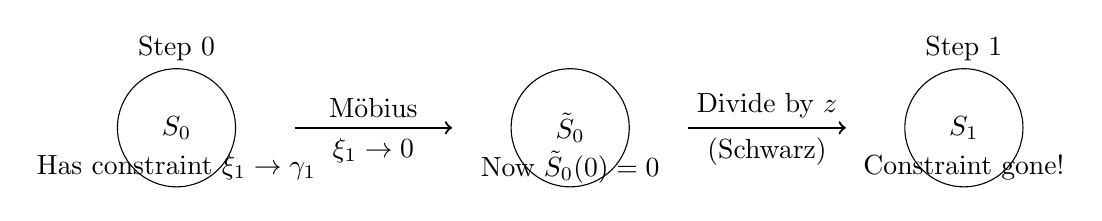
\begin{tikzpicture}
        % Step 1
        \node (S0) at (0,0) [circle, draw, minimum size=1.5cm] {$S_0$};
        \node [above of=S0] {Step 0};
        \node [below of=S0, yshift=0.5cm] {Has constraint $\xi_1 \to \gamma_1$};
        
        \draw [->, thick] (1.5,0) -- node[above] {Möbius} node[below] {$\xi_1 \to 0$} (3.5,0);
        
        % Step 2
        \node (S0_tilde) at (5,0) [circle, draw, minimum size=1.5cm] {$\tilde{S}_0$};
        \node [below of=S0_tilde, yshift=0.5cm] {Now $\tilde{S}_0(0) = 0$};
        
        \draw [->, thick] (6.5,0) -- node[above] {Divide by $z$} node[below] {(Schwarz)} (8.5,0);
        
        % Step 3
        \node (S1) at (10,0) [circle, draw, minimum size=1.5cm] {$S_1$};
        \node [below of=S1, yshift=0.5cm] {Constraint gone!};
        \node [above of=S1] {Step 1};
    \end{tikzpicture}
    
    \vspace{0.5cm}
    By repeating this, we "peel off" every data point $\xi_n$, storing the information in the transformation parameters ($\phi_n$), until no constraints remain.
\end{frame}

\begin{frame}{5.3 Forward Recursion (The Formula)}
    Let $S_k(\xi)$ be the function at step $k$. We start with $S_0(\xi) = S(\xi)$.
    
    \textbf{Iterative Process:}
    For each data point $k = 1 \dots M$:
    \begin{enumerate}
        \item \textbf{Evaluate:} The value to interpolate is $\phi_k = S_{k-1}(\xi_k)$.
        \item \textbf{Sanity Check:} If $|\phi_k| > 1$, the data is unphysical (violates causality). Stop.
        \item \textbf{Peel:} Compute the next function $S_k(\xi)$ by removing the zero at $\xi_k$:
        $$ S_k(\xi) = \frac{1}{B_k(\xi)} \frac{S_{k-1}(\xi) - \phi_k}{1 - \bar{\phi}_k S_{k-1}(\xi)} $$
    \end{enumerate}
    
    Here, $B_k(\xi) = \frac{\xi - \xi_k}{1 - \bar{\xi}_k \xi}$ is the Blaschke factor that acts like "$z$" in the Schwarz Lemma.
\end{frame}

\begin{frame}{5.4 The Free Function (Closing the Loop)}
    After matching all $M$ data points, we arrive at a function $S_M(\xi)$.
    
    \begin{itemize}
        \item Since all constraints are satisfied, $S_M(\xi)$ can be \textbf{any} contractive analytic function.
        \item We call $S_M(\xi)$ the \textbf{Free Function} $\theta(\xi)$.
    \end{itemize}
    
    \textbf{Physical Implications:}
    \begin{itemize}
        \item Setting $\theta(\xi) = 0$ yields the "simplest" solution (analytic center).
        \item We can optimize $\theta(\xi)$ to enforce additional physical priors (e.g., smoothness, sum rules) without violating the experimental data bounds.
    \end{itemize}
\end{frame}

% Section 6: Reconstruction (Original Section 4)
\subsection{Reconstruction and Summary}

\begin{frame}{6.1 Backward Reconstruction}
    To get the spectrum $A(\omega)$, we evaluate our solution on the real axis.
    
    1. Choose real frequencies $\omega$.
    2. Map to the disk boundary: $\xi = \frac{\omega - i}{\omega + i}$.
    3. Start with the free function (e.g., $S_{out} = 0$).
    4. Apply the inverse Möbius transforms in reverse order ($k=M \to 1$):
    
    \begin{equation}
        S_{out}(\xi) \leftarrow \frac{\phi_k + S_{out}(\xi) B_k(\xi)}{1 + \bar{\phi}_k S_{out}(\xi) B_k(\xi)}
    \end{equation}
    
    5. Map back to Green's function $G(\omega)$ and take the imaginary part.
\end{frame}

\begin{frame}{Summary of the Nevanlinna Workflow}
    \centering
    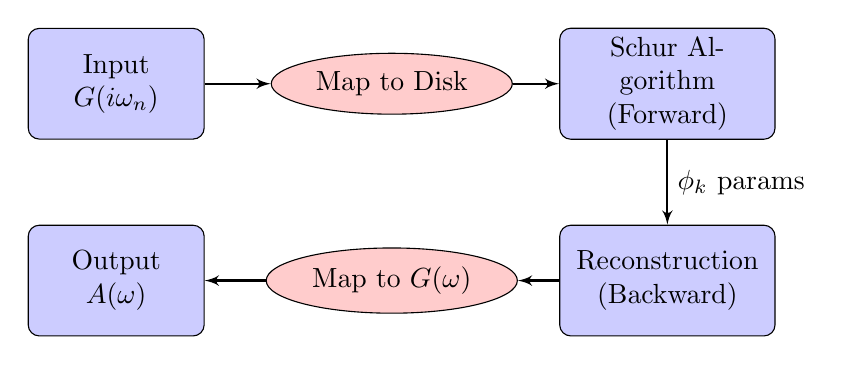
\begin{tikzpicture}[node distance=2.5cm, auto]
        % Nodes
        \node [block, text width=2cm, align=center] (input) {Input $G(i\omega_n)$};
        \node [cloud, right of=input, node distance=3.5cm] (map) {Map to Disk};
        \node [block, right of=map, node distance=3.5cm, text width=2.5cm, align=center] (schur) {Schur Algorithm (Forward)};
        \node [block, below of=schur, text width=2.5cm, align=center] (recon) {Reconstruction (Backward)};
        \node [cloud, left of=recon, node distance=3.5cm] (unmap) {Map to $G(\omega)$};
        \node [block, left of=unmap, node distance=3.5cm, text width=2cm, align=center] (output) {Output $A(\omega)$};

        % Edges
        \path [line] (input) -- (map);
        \path [line] (map) -- (schur);
        \path [line] (schur) -- node [right] {$\phi_k$ params} (recon);
        \path [line] (recon) -- (unmap);
        \path [line] (unmap) -- (output);
    \end{tikzpicture}
    
    \vspace{0.5cm}
    \begin{itemize}
        \item \textbf{Key Takeaway:} We replace ill-conditioned fitting with stable algebraic recursion.
        \item \textbf{Guarantee:} The result is always causal ($A(\omega) \ge 0$).
    \end{itemize}
\end{frame}

% Section 7: Proposed Neural Framework (Original Section 5)
\subsection{Project B: Neural Nevanlinna Framework}

\begin{frame}{7.1 The Noise Barrier in Multi-Orbital Systems}
    While Nevanlinna theory guarantees causality, the practical implementation relies on optimization to handle noise.
    
    \begin{alertblock}{The Challenge}
        \begin{itemize}
            \item \textbf{Correlated Noise:} QMC noise is highly correlated across imaginary time slices (off-diagonal covariance).
            \item \textbf{Optimization Landscape:} The standard Nevanlinna optimization is sensitive to this noise, often misinterpreting it as physical signal.
            \item \textbf{Result:} Difficulty distinguishing coherent quasiparticles from incoherent sidebands in complex materials like Strontium Ruthenate ($Sr_2RuO_4$).
        \end{itemize}
    \end{alertblock}
\end{frame}

\begin{frame}{7.2 The Proposed Solution: Neural Nevanlinna}
    We propose replacing the brittle optimization step with a robust \textbf{Neural Network}.
    
    \textbf{Core Innovation:}
    Instead of predicting the spectrum $A(\omega)$ directly (which might violate sum rules), the network predicts the \textbf{Schur parameters} $\phi_k$.
    
    \begin{itemize}
        \item \textbf{Input:} Noisy Green's function $G(i\omega_n)$.
        \item \textbf{Output:} Schur parameters $\phi_k$ (where $|\phi_k| \le 1$).
        \item \textbf{Physics Constraint:} By reconstructing $A(\omega)$ from $\phi_k$ using the analytic backward recursion, causality and positivity are enforced \textbf{by construction}.
    \end{itemize}
\end{frame}

\begin{frame}{7.3 Implementation Pipeline}
    \centering
    % Increased global node distance significantly to lengthen arrows
    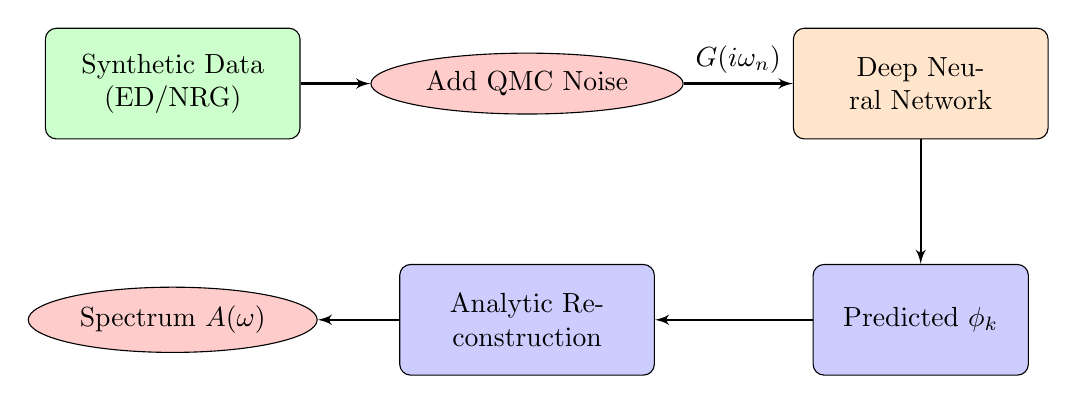
\begin{tikzpicture}[node distance=  5cm, auto] 
        % Nodes - Top Row
        \node [block, fill=green!20, text width=3cm] (data) {Synthetic Data (ED/NRG)};
        \node [cloud, right of=data, node distance=4.5cm] (noise) {Add QMC Noise};
        \node [block, right of=noise, fill=orange!20, text width=3cm] (nn) {Deep Neural Network};
        
        % Nodes - Bottom Row
        \node [block, below of=nn, node distance=3cm, text width=2.5cm] (params) {Predicted $\phi_k$};
        \node [block, left of=params, fill=blue!20, text width=3cm] (math) {Analytic Reconstruction};
        \node [cloud, left of=math, node distance=4.5cm] (spec) {Spectrum $A(\omega)$};

        % Edges
        \path [line] (data) -- (noise);
        \path [line] (noise) -- node[above] {$G(i\omega_n)$} (nn);
        \path [line] (nn) -- (params);
        \path [line] (params) -- (math);
        \path [line] (math) -- (spec);
    \end{tikzpicture}
    
    \vspace{0.2cm}
    \textbf{Strategy:} Train on synthetic data (e.g., $Sr_2RuO_4$ model) to learn the mapping from noisy inputs to the stable Schur manifold.
\end{frame}

\end{document}